% Created by tikzDevice version 0.12.6 on 2025-07-29 10:11:47
% !TEX encoding = UTF-8 Unicode
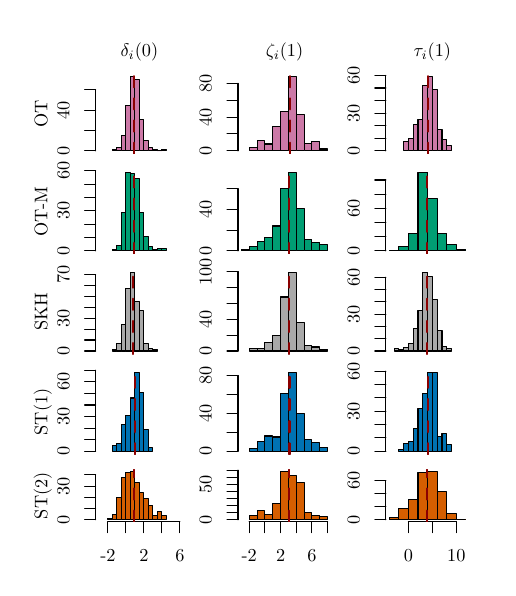
\begin{tikzpicture}[x=1pt,y=1pt]
\definecolor{fillColor}{RGB}{255,255,255}
\path[use as bounding box,fill=fillColor,fill opacity=0.00] (0,0) rectangle (166.22,195.13);
\begin{scope}
\path[clip] ( 24.55,149.59) rectangle ( 56.20,178.50);
\definecolor{drawColor}{RGB}{0,0,0}
\definecolor{fillColor}{RGB}{204,121,167}

\path[draw=drawColor,line width= 0.4pt,line join=round,line cap=round,fill=fillColor] ( 30.61,150.66) rectangle ( 32.24,151.03);

\path[draw=drawColor,line width= 0.4pt,line join=round,line cap=round,fill=fillColor] ( 32.24,150.66) rectangle ( 33.86,151.76);

\path[draw=drawColor,line width= 0.4pt,line join=round,line cap=round,fill=fillColor] ( 33.86,150.66) rectangle ( 35.49,156.16);

\path[draw=drawColor,line width= 0.4pt,line join=round,line cap=round,fill=fillColor] ( 35.49,150.66) rectangle ( 37.12,167.16);

\path[draw=drawColor,line width= 0.4pt,line join=round,line cap=round,fill=fillColor] ( 37.12,150.66) rectangle ( 38.75,177.43);

\path[draw=drawColor,line width= 0.4pt,line join=round,line cap=round,fill=fillColor] ( 38.75,150.66) rectangle ( 40.37,176.33);

\path[draw=drawColor,line width= 0.4pt,line join=round,line cap=round,fill=fillColor] ( 40.37,150.66) rectangle ( 42.00,162.03);

\path[draw=drawColor,line width= 0.4pt,line join=round,line cap=round,fill=fillColor] ( 42.00,150.66) rectangle ( 43.63,154.33);

\path[draw=drawColor,line width= 0.4pt,line join=round,line cap=round,fill=fillColor] ( 43.63,150.66) rectangle ( 45.26,151.76);

\path[draw=drawColor,line width= 0.4pt,line join=round,line cap=round,fill=fillColor] ( 45.26,150.66) rectangle ( 46.89,151.03);

\path[draw=drawColor,line width= 0.4pt,line join=round,line cap=round,fill=fillColor] ( 46.89,150.66) rectangle ( 48.51,150.66);

\path[draw=drawColor,line width= 0.4pt,line join=round,line cap=round,fill=fillColor] ( 48.51,150.66) rectangle ( 50.14,151.03);
\end{scope}
\begin{scope}
\path[clip] (  0.00,  0.00) rectangle (166.22,195.13);
\definecolor{drawColor}{RGB}{0,0,0}

\path[draw=drawColor,line width= 0.4pt,line join=round,line cap=round] ( 24.55,150.66) -- ( 24.55,172.66);

\path[draw=drawColor,line width= 0.4pt,line join=round,line cap=round] ( 24.55,150.66) -- ( 20.59,150.66);

\path[draw=drawColor,line width= 0.4pt,line join=round,line cap=round] ( 24.55,157.99) -- ( 20.59,157.99);

\path[draw=drawColor,line width= 0.4pt,line join=round,line cap=round] ( 24.55,165.33) -- ( 20.59,165.33);

\path[draw=drawColor,line width= 0.4pt,line join=round,line cap=round] ( 24.55,172.66) -- ( 20.59,172.66);

\node[text=drawColor,rotate= 90.00,anchor=base,inner sep=0pt, outer sep=0pt, scale=  0.66] at ( 15.05,150.66) {0};

\node[text=drawColor,rotate= 90.00,anchor=base,inner sep=0pt, outer sep=0pt, scale=  0.66] at ( 15.05,165.33) {40};
\end{scope}
\begin{scope}
\path[clip] (  0.00,144.84) rectangle ( 59.36,195.13);
\definecolor{drawColor}{RGB}{0,0,0}

\node[text=drawColor,anchor=base,inner sep=0pt, outer sep=0pt, scale=  0.66] at ( 40.37,184.54) {\bfseries $\delta_i(0)$};

\node[text=drawColor,rotate= 90.00,anchor=base,inner sep=0pt, outer sep=0pt, scale=  0.66] at (  7.13,164.04) {OT};
\end{scope}
\begin{scope}
\path[clip] ( 24.55,149.59) rectangle ( 56.20,178.50);
\definecolor{drawColor}{RGB}{139,0,0}

\path[draw=drawColor,line width= 0.8pt,dash pattern=on 4pt off 4pt ,line join=round,line cap=round] ( 38.56,149.59) -- ( 38.56,178.50);
\end{scope}
\begin{scope}
\path[clip] ( 76.00,149.59) rectangle (109.62,178.50);
\definecolor{drawColor}{RGB}{0,0,0}
\definecolor{fillColor}{RGB}{204,121,167}

\path[draw=drawColor,line width= 0.4pt,line join=round,line cap=round,fill=fillColor] ( 80.07,150.66) rectangle ( 82.90,151.88);

\path[draw=drawColor,line width= 0.4pt,line join=round,line cap=round,fill=fillColor] ( 82.90,150.66) rectangle ( 85.73,154.31);

\path[draw=drawColor,line width= 0.4pt,line join=round,line cap=round,fill=fillColor] ( 85.73,150.66) rectangle ( 88.56,153.09);

\path[draw=drawColor,line width= 0.4pt,line join=round,line cap=round,fill=fillColor] ( 88.56,150.66) rectangle ( 91.40,159.48);

\path[draw=drawColor,line width= 0.4pt,line join=round,line cap=round,fill=fillColor] ( 91.40,150.66) rectangle ( 94.23,164.96);

\path[draw=drawColor,line width= 0.4pt,line join=round,line cap=round,fill=fillColor] ( 94.23,150.66) rectangle ( 97.06,177.43);

\path[draw=drawColor,line width= 0.4pt,line join=round,line cap=round,fill=fillColor] ( 97.06,150.66) rectangle ( 99.89,163.74);

\path[draw=drawColor,line width= 0.4pt,line join=round,line cap=round,fill=fillColor] ( 99.89,150.66) rectangle (102.72,153.40);

\path[draw=drawColor,line width= 0.4pt,line join=round,line cap=round,fill=fillColor] (102.72,150.66) rectangle (105.55,154.01);

\path[draw=drawColor,line width= 0.4pt,line join=round,line cap=round,fill=fillColor] (105.55,150.66) rectangle (108.38,151.27);
\end{scope}
\begin{scope}
\path[clip] (  0.00,  0.00) rectangle (166.22,195.13);
\definecolor{drawColor}{RGB}{0,0,0}

\path[draw=drawColor,line width= 0.4pt,line join=round,line cap=round] ( 76.00,150.66) -- ( 76.00,174.99);

\path[draw=drawColor,line width= 0.4pt,line join=round,line cap=round] ( 76.00,150.66) -- ( 72.04,150.66);

\path[draw=drawColor,line width= 0.4pt,line join=round,line cap=round] ( 76.00,156.74) -- ( 72.04,156.74);

\path[draw=drawColor,line width= 0.4pt,line join=round,line cap=round] ( 76.00,162.83) -- ( 72.04,162.83);

\path[draw=drawColor,line width= 0.4pt,line join=round,line cap=round] ( 76.00,168.91) -- ( 72.04,168.91);

\path[draw=drawColor,line width= 0.4pt,line join=round,line cap=round] ( 76.00,174.99) -- ( 72.04,174.99);

\node[text=drawColor,rotate= 90.00,anchor=base,inner sep=0pt, outer sep=0pt, scale=  0.66] at ( 66.49,150.66) {0};

\node[text=drawColor,rotate= 90.00,anchor=base,inner sep=0pt, outer sep=0pt, scale=  0.66] at ( 66.49,162.83) {40};

\node[text=drawColor,rotate= 90.00,anchor=base,inner sep=0pt, outer sep=0pt, scale=  0.66] at ( 66.49,174.99) {80};
\end{scope}
\begin{scope}
\path[clip] ( 59.36,144.84) rectangle (112.79,195.13);
\definecolor{drawColor}{RGB}{0,0,0}

\node[text=drawColor,anchor=base,inner sep=0pt, outer sep=0pt, scale=  0.66] at ( 92.81,184.54) {\bfseries $\zeta_i(1)$};
\end{scope}
\begin{scope}
\path[clip] ( 76.00,149.59) rectangle (109.62,178.50);
\definecolor{drawColor}{RGB}{139,0,0}

\path[draw=drawColor,line width= 0.8pt,dash pattern=on 4pt off 4pt ,line join=round,line cap=round] ( 94.66,149.59) -- ( 94.66,178.50);
\end{scope}
\begin{scope}
\path[clip] (129.42,149.59) rectangle (163.05,178.50);
\definecolor{drawColor}{RGB}{0,0,0}
\definecolor{fillColor}{RGB}{204,121,167}

\path[draw=drawColor,line width= 0.4pt,line join=round,line cap=round,fill=fillColor] (135.86,150.66) rectangle (137.59,153.84);

\path[draw=drawColor,line width= 0.4pt,line join=round,line cap=round,fill=fillColor] (137.59,150.66) rectangle (139.32,155.20);

\path[draw=drawColor,line width= 0.4pt,line join=round,line cap=round,fill=fillColor] (139.32,150.66) rectangle (141.05,160.19);

\path[draw=drawColor,line width= 0.4pt,line join=round,line cap=round,fill=fillColor] (141.05,150.66) rectangle (142.78,162.00);

\path[draw=drawColor,line width= 0.4pt,line join=round,line cap=round,fill=fillColor] (142.78,150.66) rectangle (144.51,174.25);

\path[draw=drawColor,line width= 0.4pt,line join=round,line cap=round,fill=fillColor] (144.51,150.66) rectangle (146.24,177.43);

\path[draw=drawColor,line width= 0.4pt,line join=round,line cap=round,fill=fillColor] (146.24,150.66) rectangle (147.97,172.89);

\path[draw=drawColor,line width= 0.4pt,line join=round,line cap=round,fill=fillColor] (147.97,150.66) rectangle (149.70,158.37);

\path[draw=drawColor,line width= 0.4pt,line join=round,line cap=round,fill=fillColor] (149.70,150.66) rectangle (151.43,154.74);

\path[draw=drawColor,line width= 0.4pt,line join=round,line cap=round,fill=fillColor] (151.43,150.66) rectangle (153.16,152.48);
\end{scope}
\begin{scope}
\path[clip] (  0.00,  0.00) rectangle (166.22,195.13);
\definecolor{drawColor}{RGB}{0,0,0}

\path[draw=drawColor,line width= 0.4pt,line join=round,line cap=round] (129.42,150.66) -- (129.42,177.88);

\path[draw=drawColor,line width= 0.4pt,line join=round,line cap=round] (129.42,150.66) -- (125.46,150.66);

\path[draw=drawColor,line width= 0.4pt,line join=round,line cap=round] (129.42,155.20) -- (125.46,155.20);

\path[draw=drawColor,line width= 0.4pt,line join=round,line cap=round] (129.42,159.73) -- (125.46,159.73);

\path[draw=drawColor,line width= 0.4pt,line join=round,line cap=round] (129.42,164.27) -- (125.46,164.27);

\path[draw=drawColor,line width= 0.4pt,line join=round,line cap=round] (129.42,168.81) -- (125.46,168.81);

\path[draw=drawColor,line width= 0.4pt,line join=round,line cap=round] (129.42,173.34) -- (125.46,173.34);

\path[draw=drawColor,line width= 0.4pt,line join=round,line cap=round] (129.42,177.88) -- (125.46,177.88);

\node[text=drawColor,rotate= 90.00,anchor=base,inner sep=0pt, outer sep=0pt, scale=  0.66] at (119.92,150.66) {0};

\node[text=drawColor,rotate= 90.00,anchor=base,inner sep=0pt, outer sep=0pt, scale=  0.66] at (119.92,164.27) {30};

\node[text=drawColor,rotate= 90.00,anchor=base,inner sep=0pt, outer sep=0pt, scale=  0.66] at (119.92,177.88) {60};
\end{scope}
\begin{scope}
\path[clip] (112.79,144.84) rectangle (166.22,195.13);
\definecolor{drawColor}{RGB}{0,0,0}

\node[text=drawColor,anchor=base,inner sep=0pt, outer sep=0pt, scale=  0.66] at (146.24,184.54) {\bfseries $\tau_i(1)$};
\end{scope}
\begin{scope}
\path[clip] (129.42,149.59) rectangle (163.05,178.50);
\definecolor{drawColor}{RGB}{139,0,0}

\path[draw=drawColor,line width= 0.8pt,dash pattern=on 4pt off 4pt ,line join=round,line cap=round] (144.67,149.59) -- (144.67,178.50);
\end{scope}
\begin{scope}
\path[clip] ( 24.55,113.38) rectangle ( 56.20,144.05);
\definecolor{drawColor}{RGB}{0,0,0}
\definecolor{fillColor}{RGB}{0,158,115}

\path[draw=drawColor,line width= 0.4pt,line join=round,line cap=round,fill=fillColor] ( 30.61,114.52) rectangle ( 32.24,115.00);

\path[draw=drawColor,line width= 0.4pt,line join=round,line cap=round,fill=fillColor] ( 32.24,114.52) rectangle ( 33.86,116.44);

\path[draw=drawColor,line width= 0.4pt,line join=round,line cap=round,fill=fillColor] ( 33.86,114.52) rectangle ( 35.49,128.47);

\path[draw=drawColor,line width= 0.4pt,line join=round,line cap=round,fill=fillColor] ( 35.49,114.52) rectangle ( 37.12,142.91);

\path[draw=drawColor,line width= 0.4pt,line join=round,line cap=round,fill=fillColor] ( 37.12,114.52) rectangle ( 38.75,142.43);

\path[draw=drawColor,line width= 0.4pt,line join=round,line cap=round,fill=fillColor] ( 38.75,114.52) rectangle ( 40.37,140.50);

\path[draw=drawColor,line width= 0.4pt,line join=round,line cap=round,fill=fillColor] ( 40.37,114.52) rectangle ( 42.00,128.47);

\path[draw=drawColor,line width= 0.4pt,line join=round,line cap=round,fill=fillColor] ( 42.00,114.52) rectangle ( 43.63,119.81);

\path[draw=drawColor,line width= 0.4pt,line join=round,line cap=round,fill=fillColor] ( 43.63,114.52) rectangle ( 45.26,115.96);

\path[draw=drawColor,line width= 0.4pt,line join=round,line cap=round,fill=fillColor] ( 45.26,114.52) rectangle ( 46.89,115.00);

\path[draw=drawColor,line width= 0.4pt,line join=round,line cap=round,fill=fillColor] ( 46.89,114.52) rectangle ( 48.51,115.48);

\path[draw=drawColor,line width= 0.4pt,line join=round,line cap=round,fill=fillColor] ( 48.51,114.52) rectangle ( 50.14,115.48);
\end{scope}
\begin{scope}
\path[clip] (  0.00,  0.00) rectangle (166.22,195.13);
\definecolor{drawColor}{RGB}{0,0,0}

\path[draw=drawColor,line width= 0.4pt,line join=round,line cap=round] ( 24.55,114.52) -- ( 24.55,143.39);

\path[draw=drawColor,line width= 0.4pt,line join=round,line cap=round] ( 24.55,114.52) -- ( 20.59,114.52);

\path[draw=drawColor,line width= 0.4pt,line join=round,line cap=round] ( 24.55,119.33) -- ( 20.59,119.33);

\path[draw=drawColor,line width= 0.4pt,line join=round,line cap=round] ( 24.55,124.14) -- ( 20.59,124.14);

\path[draw=drawColor,line width= 0.4pt,line join=round,line cap=round] ( 24.55,128.95) -- ( 20.59,128.95);

\path[draw=drawColor,line width= 0.4pt,line join=round,line cap=round] ( 24.55,133.77) -- ( 20.59,133.77);

\path[draw=drawColor,line width= 0.4pt,line join=round,line cap=round] ( 24.55,138.58) -- ( 20.59,138.58);

\path[draw=drawColor,line width= 0.4pt,line join=round,line cap=round] ( 24.55,143.39) -- ( 20.59,143.39);

\node[text=drawColor,rotate= 90.00,anchor=base,inner sep=0pt, outer sep=0pt, scale=  0.66] at ( 15.05,114.52) {0};

\node[text=drawColor,rotate= 90.00,anchor=base,inner sep=0pt, outer sep=0pt, scale=  0.66] at ( 15.05,128.95) {30};

\node[text=drawColor,rotate= 90.00,anchor=base,inner sep=0pt, outer sep=0pt, scale=  0.66] at ( 15.05,143.39) {60};
\end{scope}
\begin{scope}
\path[clip] (  0.00,108.63) rectangle ( 59.36,144.84);
\definecolor{drawColor}{RGB}{0,0,0}

\node[text=drawColor,rotate= 90.00,anchor=base,inner sep=0pt, outer sep=0pt, scale=  0.66] at (  7.13,128.71) {OT-M};
\end{scope}
\begin{scope}
\path[clip] ( 24.55,113.38) rectangle ( 56.20,144.05);
\definecolor{drawColor}{RGB}{139,0,0}

\path[draw=drawColor,line width= 0.8pt,dash pattern=on 4pt off 4pt ,line join=round,line cap=round] ( 38.30,113.38) -- ( 38.30,144.05);
\end{scope}
\begin{scope}
\path[clip] ( 76.00,113.38) rectangle (109.62,144.05);
\definecolor{drawColor}{RGB}{0,0,0}
\definecolor{fillColor}{RGB}{0,158,115}

\path[draw=drawColor,line width= 0.4pt,line join=round,line cap=round,fill=fillColor] ( 77.24,114.52) rectangle ( 80.07,114.89);

\path[draw=drawColor,line width= 0.4pt,line join=round,line cap=round,fill=fillColor] ( 80.07,114.52) rectangle ( 82.90,116.01);

\path[draw=drawColor,line width= 0.4pt,line join=round,line cap=round,fill=fillColor] ( 82.90,114.52) rectangle ( 85.73,117.88);

\path[draw=drawColor,line width= 0.4pt,line join=round,line cap=round,fill=fillColor] ( 85.73,114.52) rectangle ( 88.56,119.37);

\path[draw=drawColor,line width= 0.4pt,line join=round,line cap=round,fill=fillColor] ( 88.56,114.52) rectangle ( 91.40,123.48);

\path[draw=drawColor,line width= 0.4pt,line join=round,line cap=round,fill=fillColor] ( 91.40,114.52) rectangle ( 94.23,136.93);

\path[draw=drawColor,line width= 0.4pt,line join=round,line cap=round,fill=fillColor] ( 94.23,114.52) rectangle ( 97.06,142.91);

\path[draw=drawColor,line width= 0.4pt,line join=round,line cap=round,fill=fillColor] ( 97.06,114.52) rectangle ( 99.89,129.83);

\path[draw=drawColor,line width= 0.4pt,line join=round,line cap=round,fill=fillColor] ( 99.89,114.52) rectangle (102.72,118.63);

\path[draw=drawColor,line width= 0.4pt,line join=round,line cap=round,fill=fillColor] (102.72,114.52) rectangle (105.55,117.51);

\path[draw=drawColor,line width= 0.4pt,line join=round,line cap=round,fill=fillColor] (105.55,114.52) rectangle (108.38,116.76);
\end{scope}
\begin{scope}
\path[clip] (  0.00,  0.00) rectangle (166.22,195.13);
\definecolor{drawColor}{RGB}{0,0,0}

\path[draw=drawColor,line width= 0.4pt,line join=round,line cap=round] ( 76.00,114.52) -- ( 76.00,136.93);

\path[draw=drawColor,line width= 0.4pt,line join=round,line cap=round] ( 76.00,114.52) -- ( 72.04,114.52);

\path[draw=drawColor,line width= 0.4pt,line join=round,line cap=round] ( 76.00,121.99) -- ( 72.04,121.99);

\path[draw=drawColor,line width= 0.4pt,line join=round,line cap=round] ( 76.00,129.46) -- ( 72.04,129.46);

\path[draw=drawColor,line width= 0.4pt,line join=round,line cap=round] ( 76.00,136.93) -- ( 72.04,136.93);

\node[text=drawColor,rotate= 90.00,anchor=base,inner sep=0pt, outer sep=0pt, scale=  0.66] at ( 66.49,114.52) {0};

\node[text=drawColor,rotate= 90.00,anchor=base,inner sep=0pt, outer sep=0pt, scale=  0.66] at ( 66.49,129.46) {40};
\end{scope}
\begin{scope}
\path[clip] ( 76.00,113.38) rectangle (109.62,144.05);
\definecolor{drawColor}{RGB}{139,0,0}

\path[draw=drawColor,line width= 0.8pt,dash pattern=on 4pt off 4pt ,line join=round,line cap=round] ( 94.44,113.38) -- ( 94.44,144.05);
\end{scope}
\begin{scope}
\path[clip] (129.42,113.38) rectangle (163.05,144.05);
\definecolor{drawColor}{RGB}{0,0,0}
\definecolor{fillColor}{RGB}{0,158,115}

\path[draw=drawColor,line width= 0.4pt,line join=round,line cap=round,fill=fillColor] (130.67,114.52) rectangle (134.13,114.77);

\path[draw=drawColor,line width= 0.4pt,line join=round,line cap=round,fill=fillColor] (134.13,114.52) rectangle (137.59,116.05);

\path[draw=drawColor,line width= 0.4pt,line join=round,line cap=round,fill=fillColor] (137.59,114.52) rectangle (141.05,120.91);

\path[draw=drawColor,line width= 0.4pt,line join=round,line cap=round,fill=fillColor] (141.05,114.52) rectangle (144.51,142.91);

\path[draw=drawColor,line width= 0.4pt,line join=round,line cap=round,fill=fillColor] (144.51,114.52) rectangle (147.97,133.45);

\path[draw=drawColor,line width= 0.4pt,line join=round,line cap=round,fill=fillColor] (147.97,114.52) rectangle (151.43,120.91);

\path[draw=drawColor,line width= 0.4pt,line join=round,line cap=round,fill=fillColor] (151.43,114.52) rectangle (154.89,116.82);

\path[draw=drawColor,line width= 0.4pt,line join=round,line cap=round,fill=fillColor] (154.89,114.52) rectangle (158.35,115.03);
\end{scope}
\begin{scope}
\path[clip] (  0.00,  0.00) rectangle (166.22,195.13);
\definecolor{drawColor}{RGB}{0,0,0}

\path[draw=drawColor,line width= 0.4pt,line join=round,line cap=round] (129.42,114.52) -- (129.42,140.10);

\path[draw=drawColor,line width= 0.4pt,line join=round,line cap=round] (129.42,114.52) -- (125.46,114.52);

\path[draw=drawColor,line width= 0.4pt,line join=round,line cap=round] (129.42,119.63) -- (125.46,119.63);

\path[draw=drawColor,line width= 0.4pt,line join=round,line cap=round] (129.42,124.75) -- (125.46,124.75);

\path[draw=drawColor,line width= 0.4pt,line join=round,line cap=round] (129.42,129.86) -- (125.46,129.86);

\path[draw=drawColor,line width= 0.4pt,line join=round,line cap=round] (129.42,134.98) -- (125.46,134.98);

\path[draw=drawColor,line width= 0.4pt,line join=round,line cap=round] (129.42,140.10) -- (125.46,140.10);

\node[text=drawColor,rotate= 90.00,anchor=base,inner sep=0pt, outer sep=0pt, scale=  0.66] at (119.92,114.52) {0};

\node[text=drawColor,rotate= 90.00,anchor=base,inner sep=0pt, outer sep=0pt, scale=  0.66] at (119.92,129.86) {60};
\end{scope}
\begin{scope}
\path[clip] (129.42,113.38) rectangle (163.05,144.05);
\definecolor{drawColor}{RGB}{139,0,0}

\path[draw=drawColor,line width= 0.8pt,dash pattern=on 4pt off 4pt ,line join=round,line cap=round] (144.40,113.38) -- (144.40,144.05);
\end{scope}
\begin{scope}
\path[clip] ( 24.55, 77.17) rectangle ( 56.20,107.84);
\definecolor{drawColor}{RGB}{0,0,0}
\definecolor{fillColor}{RGB}{169,169,169}

\path[draw=drawColor,line width= 0.4pt,line join=round,line cap=round,fill=fillColor] ( 30.61, 78.31) rectangle ( 32.24, 78.70);

\path[draw=drawColor,line width= 0.4pt,line join=round,line cap=round,fill=fillColor] ( 32.24, 78.31) rectangle ( 33.86, 81.07);

\path[draw=drawColor,line width= 0.4pt,line join=round,line cap=round,fill=fillColor] ( 33.86, 78.31) rectangle ( 35.49, 87.77);

\path[draw=drawColor,line width= 0.4pt,line join=round,line cap=round,fill=fillColor] ( 35.49, 78.31) rectangle ( 37.12,100.79);

\path[draw=drawColor,line width= 0.4pt,line join=round,line cap=round,fill=fillColor] ( 37.12, 78.31) rectangle ( 38.75,106.70);

\path[draw=drawColor,line width= 0.4pt,line join=round,line cap=round,fill=fillColor] ( 38.75, 78.31) rectangle ( 40.37, 96.05);

\path[draw=drawColor,line width= 0.4pt,line join=round,line cap=round,fill=fillColor] ( 40.37, 78.31) rectangle ( 42.00, 92.90);

\path[draw=drawColor,line width= 0.4pt,line join=round,line cap=round,fill=fillColor] ( 42.00, 78.31) rectangle ( 43.63, 81.07);

\path[draw=drawColor,line width= 0.4pt,line join=round,line cap=round,fill=fillColor] ( 43.63, 78.31) rectangle ( 45.26, 79.10);

\path[draw=drawColor,line width= 0.4pt,line join=round,line cap=round,fill=fillColor] ( 45.26, 78.31) rectangle ( 46.89, 78.70);
\end{scope}
\begin{scope}
\path[clip] (  0.00,  0.00) rectangle (166.22,195.13);
\definecolor{drawColor}{RGB}{0,0,0}

\path[draw=drawColor,line width= 0.4pt,line join=round,line cap=round] ( 24.55, 78.31) -- ( 24.55,105.91);

\path[draw=drawColor,line width= 0.4pt,line join=round,line cap=round] ( 24.55, 78.31) -- ( 20.59, 78.31);

\path[draw=drawColor,line width= 0.4pt,line join=round,line cap=round] ( 24.55, 82.25) -- ( 20.59, 82.25);

\path[draw=drawColor,line width= 0.4pt,line join=round,line cap=round] ( 24.55, 86.19) -- ( 20.59, 86.19);

\path[draw=drawColor,line width= 0.4pt,line join=round,line cap=round] ( 24.55, 90.14) -- ( 20.59, 90.14);

\path[draw=drawColor,line width= 0.4pt,line join=round,line cap=round] ( 24.55, 94.08) -- ( 20.59, 94.08);

\path[draw=drawColor,line width= 0.4pt,line join=round,line cap=round] ( 24.55, 98.02) -- ( 20.59, 98.02);

\path[draw=drawColor,line width= 0.4pt,line join=round,line cap=round] ( 24.55,101.97) -- ( 20.59,101.97);

\path[draw=drawColor,line width= 0.4pt,line join=round,line cap=round] ( 24.55,105.91) -- ( 20.59,105.91);

\node[text=drawColor,rotate= 90.00,anchor=base,inner sep=0pt, outer sep=0pt, scale=  0.66] at ( 15.05, 78.31) {0};

\node[text=drawColor,rotate= 90.00,anchor=base,inner sep=0pt, outer sep=0pt, scale=  0.66] at ( 15.05, 90.14) {30};

\node[text=drawColor,rotate= 90.00,anchor=base,inner sep=0pt, outer sep=0pt, scale=  0.66] at ( 15.05,105.91) {70};
\end{scope}
\begin{scope}
\path[clip] (  0.00, 72.42) rectangle ( 59.36,108.63);
\definecolor{drawColor}{RGB}{0,0,0}

\node[text=drawColor,rotate= 90.00,anchor=base,inner sep=0pt, outer sep=0pt, scale=  0.66] at (  7.13, 92.50) {SKH};
\end{scope}
\begin{scope}
\path[clip] ( 24.55, 77.17) rectangle ( 56.20,107.84);
\definecolor{drawColor}{RGB}{139,0,0}

\path[draw=drawColor,line width= 0.8pt,dash pattern=on 4pt off 4pt ,line join=round,line cap=round] ( 38.07, 77.17) -- ( 38.07,107.84);
\end{scope}
\begin{scope}
\path[clip] ( 76.00, 77.17) rectangle (109.62,107.84);
\definecolor{drawColor}{RGB}{0,0,0}
\definecolor{fillColor}{RGB}{169,169,169}

\path[draw=drawColor,line width= 0.4pt,line join=round,line cap=round,fill=fillColor] ( 80.07, 78.31) rectangle ( 82.90, 79.17);

\path[draw=drawColor,line width= 0.4pt,line join=round,line cap=round,fill=fillColor] ( 82.90, 78.31) rectangle ( 85.73, 79.17);

\path[draw=drawColor,line width= 0.4pt,line join=round,line cap=round,fill=fillColor] ( 85.73, 78.31) rectangle ( 88.56, 81.46);

\path[draw=drawColor,line width= 0.4pt,line join=round,line cap=round,fill=fillColor] ( 88.56, 78.31) rectangle ( 91.40, 83.76);

\path[draw=drawColor,line width= 0.4pt,line join=round,line cap=round,fill=fillColor] ( 91.40, 78.31) rectangle ( 94.23, 97.81);

\path[draw=drawColor,line width= 0.4pt,line join=round,line cap=round,fill=fillColor] ( 94.23, 78.31) rectangle ( 97.06,106.70);

\path[draw=drawColor,line width= 0.4pt,line join=round,line cap=round,fill=fillColor] ( 97.06, 78.31) rectangle ( 99.89, 88.63);

\path[draw=drawColor,line width= 0.4pt,line join=round,line cap=round,fill=fillColor] ( 99.89, 78.31) rectangle (102.72, 80.31);

\path[draw=drawColor,line width= 0.4pt,line join=round,line cap=round,fill=fillColor] (102.72, 78.31) rectangle (105.55, 79.74);

\path[draw=drawColor,line width= 0.4pt,line join=round,line cap=round,fill=fillColor] (105.55, 78.31) rectangle (108.38, 78.88);
\end{scope}
\begin{scope}
\path[clip] (  0.00,  0.00) rectangle (166.22,195.13);
\definecolor{drawColor}{RGB}{0,0,0}

\path[draw=drawColor,line width= 0.4pt,line join=round,line cap=round] ( 76.00, 78.31) -- ( 76.00,106.99);

\path[draw=drawColor,line width= 0.4pt,line join=round,line cap=round] ( 76.00, 78.31) -- ( 72.04, 78.31);

\path[draw=drawColor,line width= 0.4pt,line join=round,line cap=round] ( 76.00, 84.04) -- ( 72.04, 84.04);

\path[draw=drawColor,line width= 0.4pt,line join=round,line cap=round] ( 76.00, 89.78) -- ( 72.04, 89.78);

\path[draw=drawColor,line width= 0.4pt,line join=round,line cap=round] ( 76.00, 95.52) -- ( 72.04, 95.52);

\path[draw=drawColor,line width= 0.4pt,line join=round,line cap=round] ( 76.00,101.25) -- ( 72.04,101.25);

\path[draw=drawColor,line width= 0.4pt,line join=round,line cap=round] ( 76.00,106.99) -- ( 72.04,106.99);

\node[text=drawColor,rotate= 90.00,anchor=base,inner sep=0pt, outer sep=0pt, scale=  0.66] at ( 66.49, 78.31) {0};

\node[text=drawColor,rotate= 90.00,anchor=base,inner sep=0pt, outer sep=0pt, scale=  0.66] at ( 66.49, 89.78) {40};

\node[text=drawColor,rotate= 90.00,anchor=base,inner sep=0pt, outer sep=0pt, scale=  0.66] at ( 66.49,106.99) {100};
\end{scope}
\begin{scope}
\path[clip] ( 76.00, 77.17) rectangle (109.62,107.84);
\definecolor{drawColor}{RGB}{139,0,0}

\path[draw=drawColor,line width= 0.8pt,dash pattern=on 4pt off 4pt ,line join=round,line cap=round] ( 94.57, 77.17) -- ( 94.57,107.84);
\end{scope}
\begin{scope}
\path[clip] (129.42, 77.17) rectangle (163.05,107.84);
\definecolor{drawColor}{RGB}{0,0,0}
\definecolor{fillColor}{RGB}{169,169,169}

\path[draw=drawColor,line width= 0.4pt,line join=round,line cap=round,fill=fillColor] (132.40, 78.31) rectangle (134.13, 79.19);

\path[draw=drawColor,line width= 0.4pt,line join=round,line cap=round,fill=fillColor] (134.13, 78.31) rectangle (135.86, 78.75);

\path[draw=drawColor,line width= 0.4pt,line join=round,line cap=round,fill=fillColor] (135.86, 78.31) rectangle (137.59, 79.64);

\path[draw=drawColor,line width= 0.4pt,line join=round,line cap=round,fill=fillColor] (137.59, 78.31) rectangle (139.32, 80.97);

\path[draw=drawColor,line width= 0.4pt,line join=round,line cap=round,fill=fillColor] (139.32, 78.31) rectangle (141.05, 86.29);

\path[draw=drawColor,line width= 0.4pt,line join=round,line cap=round,fill=fillColor] (141.05, 78.31) rectangle (142.78, 92.95);

\path[draw=drawColor,line width= 0.4pt,line join=round,line cap=round,fill=fillColor] (142.78, 78.31) rectangle (144.51,106.70);

\path[draw=drawColor,line width= 0.4pt,line join=round,line cap=round,fill=fillColor] (144.51, 78.31) rectangle (146.24,105.37);

\path[draw=drawColor,line width= 0.4pt,line join=round,line cap=round,fill=fillColor] (146.24, 78.31) rectangle (147.97, 96.94);

\path[draw=drawColor,line width= 0.4pt,line join=round,line cap=round,fill=fillColor] (147.97, 78.31) rectangle (149.70, 85.85);

\path[draw=drawColor,line width= 0.4pt,line join=round,line cap=round,fill=fillColor] (149.70, 78.31) rectangle (151.43, 80.08);

\path[draw=drawColor,line width= 0.4pt,line join=round,line cap=round,fill=fillColor] (151.43, 78.31) rectangle (153.16, 79.19);
\end{scope}
\begin{scope}
\path[clip] (  0.00,  0.00) rectangle (166.22,195.13);
\definecolor{drawColor}{RGB}{0,0,0}

\path[draw=drawColor,line width= 0.4pt,line join=round,line cap=round] (129.42, 78.31) -- (129.42,104.93);

\path[draw=drawColor,line width= 0.4pt,line join=round,line cap=round] (129.42, 78.31) -- (125.46, 78.31);

\path[draw=drawColor,line width= 0.4pt,line join=round,line cap=round] (129.42, 82.74) -- (125.46, 82.74);

\path[draw=drawColor,line width= 0.4pt,line join=round,line cap=round] (129.42, 87.18) -- (125.46, 87.18);

\path[draw=drawColor,line width= 0.4pt,line join=round,line cap=round] (129.42, 91.62) -- (125.46, 91.62);

\path[draw=drawColor,line width= 0.4pt,line join=round,line cap=round] (129.42, 96.05) -- (125.46, 96.05);

\path[draw=drawColor,line width= 0.4pt,line join=round,line cap=round] (129.42,100.49) -- (125.46,100.49);

\path[draw=drawColor,line width= 0.4pt,line join=round,line cap=round] (129.42,104.93) -- (125.46,104.93);

\node[text=drawColor,rotate= 90.00,anchor=base,inner sep=0pt, outer sep=0pt, scale=  0.66] at (119.92, 78.31) {0};

\node[text=drawColor,rotate= 90.00,anchor=base,inner sep=0pt, outer sep=0pt, scale=  0.66] at (119.92, 91.62) {30};

\node[text=drawColor,rotate= 90.00,anchor=base,inner sep=0pt, outer sep=0pt, scale=  0.66] at (119.92,104.93) {60};
\end{scope}
\begin{scope}
\path[clip] (129.42, 77.17) rectangle (163.05,107.84);
\definecolor{drawColor}{RGB}{139,0,0}

\path[draw=drawColor,line width= 0.8pt,dash pattern=on 4pt off 4pt ,line join=round,line cap=round] (144.36, 77.17) -- (144.36,107.84);
\end{scope}
\begin{scope}
\path[clip] ( 24.55, 40.96) rectangle ( 56.20, 71.63);
\definecolor{drawColor}{RGB}{0,0,0}
\definecolor{fillColor}{RGB}{0,114,178}

\path[draw=drawColor,line width= 0.4pt,line join=round,line cap=round,fill=fillColor] ( 30.61, 42.10) rectangle ( 32.24, 44.19);

\path[draw=drawColor,line width= 0.4pt,line join=round,line cap=round,fill=fillColor] ( 32.24, 42.10) rectangle ( 33.86, 45.02);

\path[draw=drawColor,line width= 0.4pt,line join=round,line cap=round,fill=fillColor] ( 33.86, 42.10) rectangle ( 35.49, 51.70);

\path[draw=drawColor,line width= 0.4pt,line join=round,line cap=round,fill=fillColor] ( 35.49, 42.10) rectangle ( 37.12, 55.04);

\path[draw=drawColor,line width= 0.4pt,line join=round,line cap=round,fill=fillColor] ( 37.12, 42.10) rectangle ( 38.75, 61.30);

\path[draw=drawColor,line width= 0.4pt,line join=round,line cap=round,fill=fillColor] ( 38.75, 42.10) rectangle ( 40.37, 70.49);

\path[draw=drawColor,line width= 0.4pt,line join=round,line cap=round,fill=fillColor] ( 40.37, 42.10) rectangle ( 42.00, 63.39);

\path[draw=drawColor,line width= 0.4pt,line join=round,line cap=round,fill=fillColor] ( 42.00, 42.10) rectangle ( 43.63, 50.03);

\path[draw=drawColor,line width= 0.4pt,line join=round,line cap=round,fill=fillColor] ( 43.63, 42.10) rectangle ( 45.26, 43.35);
\end{scope}
\begin{scope}
\path[clip] (  0.00,  0.00) rectangle (166.22,195.13);
\definecolor{drawColor}{RGB}{0,0,0}

\path[draw=drawColor,line width= 0.4pt,line join=round,line cap=round] ( 24.55, 42.10) -- ( 24.55, 71.33);

\path[draw=drawColor,line width= 0.4pt,line join=round,line cap=round] ( 24.55, 42.10) -- ( 20.59, 42.10);

\path[draw=drawColor,line width= 0.4pt,line join=round,line cap=round] ( 24.55, 46.27) -- ( 20.59, 46.27);

\path[draw=drawColor,line width= 0.4pt,line join=round,line cap=round] ( 24.55, 50.45) -- ( 20.59, 50.45);

\path[draw=drawColor,line width= 0.4pt,line join=round,line cap=round] ( 24.55, 54.62) -- ( 20.59, 54.62);

\path[draw=drawColor,line width= 0.4pt,line join=round,line cap=round] ( 24.55, 58.80) -- ( 20.59, 58.80);

\path[draw=drawColor,line width= 0.4pt,line join=round,line cap=round] ( 24.55, 62.98) -- ( 20.59, 62.98);

\path[draw=drawColor,line width= 0.4pt,line join=round,line cap=round] ( 24.55, 67.15) -- ( 20.59, 67.15);

\path[draw=drawColor,line width= 0.4pt,line join=round,line cap=round] ( 24.55, 71.33) -- ( 20.59, 71.33);

\node[text=drawColor,rotate= 90.00,anchor=base,inner sep=0pt, outer sep=0pt, scale=  0.66] at ( 15.05, 42.10) {0};

\node[text=drawColor,rotate= 90.00,anchor=base,inner sep=0pt, outer sep=0pt, scale=  0.66] at ( 15.05, 54.62) {30};

\node[text=drawColor,rotate= 90.00,anchor=base,inner sep=0pt, outer sep=0pt, scale=  0.66] at ( 15.05, 67.15) {60};
\end{scope}
\begin{scope}
\path[clip] (  0.00, 36.21) rectangle ( 59.36, 72.42);
\definecolor{drawColor}{RGB}{0,0,0}

\node[text=drawColor,rotate= 90.00,anchor=base,inner sep=0pt, outer sep=0pt, scale=  0.66] at (  7.13, 56.29) {ST(1)};
\end{scope}
\begin{scope}
\path[clip] ( 24.55, 40.96) rectangle ( 56.20, 71.63);
\definecolor{drawColor}{RGB}{139,0,0}

\path[draw=drawColor,line width= 0.8pt,dash pattern=on 4pt off 4pt ,line join=round,line cap=round] ( 38.79, 40.96) -- ( 38.79, 71.63);
\end{scope}
\begin{scope}
\path[clip] ( 76.00, 40.96) rectangle (109.62, 71.63);
\definecolor{drawColor}{RGB}{0,0,0}
\definecolor{fillColor}{RGB}{0,114,178}

\path[draw=drawColor,line width= 0.4pt,line join=round,line cap=round,fill=fillColor] ( 80.07, 42.10) rectangle ( 82.90, 43.12);

\path[draw=drawColor,line width= 0.4pt,line join=round,line cap=round,fill=fillColor] ( 82.90, 42.10) rectangle ( 85.73, 45.52);

\path[draw=drawColor,line width= 0.4pt,line join=round,line cap=round,fill=fillColor] ( 85.73, 42.10) rectangle ( 88.56, 47.57);

\path[draw=drawColor,line width= 0.4pt,line join=round,line cap=round,fill=fillColor] ( 88.56, 42.10) rectangle ( 91.40, 47.23);

\path[draw=drawColor,line width= 0.4pt,line join=round,line cap=round,fill=fillColor] ( 91.40, 42.10) rectangle ( 94.23, 62.97);

\path[draw=drawColor,line width= 0.4pt,line join=round,line cap=round,fill=fillColor] ( 94.23, 42.10) rectangle ( 97.06, 70.49);

\path[draw=drawColor,line width= 0.4pt,line join=round,line cap=round,fill=fillColor] ( 97.06, 42.10) rectangle ( 99.89, 55.78);

\path[draw=drawColor,line width= 0.4pt,line join=round,line cap=round,fill=fillColor] ( 99.89, 42.10) rectangle (102.72, 46.20);

\path[draw=drawColor,line width= 0.4pt,line join=round,line cap=round,fill=fillColor] (102.72, 42.10) rectangle (105.55, 45.18);

\path[draw=drawColor,line width= 0.4pt,line join=round,line cap=round,fill=fillColor] (105.55, 42.10) rectangle (108.38, 43.47);
\end{scope}
\begin{scope}
\path[clip] (  0.00,  0.00) rectangle (166.22,195.13);
\definecolor{drawColor}{RGB}{0,0,0}

\path[draw=drawColor,line width= 0.4pt,line join=round,line cap=round] ( 76.00, 42.10) -- ( 76.00, 69.46);

\path[draw=drawColor,line width= 0.4pt,line join=round,line cap=round] ( 76.00, 42.10) -- ( 72.04, 42.10);

\path[draw=drawColor,line width= 0.4pt,line join=round,line cap=round] ( 76.00, 48.94) -- ( 72.04, 48.94);

\path[draw=drawColor,line width= 0.4pt,line join=round,line cap=round] ( 76.00, 55.78) -- ( 72.04, 55.78);

\path[draw=drawColor,line width= 0.4pt,line join=round,line cap=round] ( 76.00, 62.62) -- ( 72.04, 62.62);

\path[draw=drawColor,line width= 0.4pt,line join=round,line cap=round] ( 76.00, 69.46) -- ( 72.04, 69.46);

\node[text=drawColor,rotate= 90.00,anchor=base,inner sep=0pt, outer sep=0pt, scale=  0.66] at ( 66.49, 42.10) {0};

\node[text=drawColor,rotate= 90.00,anchor=base,inner sep=0pt, outer sep=0pt, scale=  0.66] at ( 66.49, 55.78) {40};

\node[text=drawColor,rotate= 90.00,anchor=base,inner sep=0pt, outer sep=0pt, scale=  0.66] at ( 66.49, 69.46) {80};
\end{scope}
\begin{scope}
\path[clip] ( 76.00, 40.96) rectangle (109.62, 71.63);
\definecolor{drawColor}{RGB}{139,0,0}

\path[draw=drawColor,line width= 0.8pt,dash pattern=on 4pt off 4pt ,line join=round,line cap=round] ( 94.62, 40.96) -- ( 94.62, 71.63);
\end{scope}
\begin{scope}
\path[clip] (129.42, 40.96) rectangle (163.05, 71.63);
\definecolor{drawColor}{RGB}{0,0,0}
\definecolor{fillColor}{RGB}{0,114,178}

\path[draw=drawColor,line width= 0.4pt,line join=round,line cap=round,fill=fillColor] (134.13, 42.10) rectangle (135.86, 42.58);

\path[draw=drawColor,line width= 0.4pt,line join=round,line cap=round,fill=fillColor] (135.86, 42.10) rectangle (137.59, 44.98);

\path[draw=drawColor,line width= 0.4pt,line join=round,line cap=round,fill=fillColor] (137.59, 42.10) rectangle (139.32, 45.47);

\path[draw=drawColor,line width= 0.4pt,line join=round,line cap=round,fill=fillColor] (139.32, 42.10) rectangle (141.05, 50.28);

\path[draw=drawColor,line width= 0.4pt,line join=round,line cap=round,fill=fillColor] (141.05, 42.10) rectangle (142.78, 57.50);

\path[draw=drawColor,line width= 0.4pt,line join=round,line cap=round,fill=fillColor] (142.78, 42.10) rectangle (144.51, 62.79);

\path[draw=drawColor,line width= 0.4pt,line join=round,line cap=round,fill=fillColor] (144.51, 42.10) rectangle (146.24, 70.49);

\path[draw=drawColor,line width= 0.4pt,line join=round,line cap=round,fill=fillColor] (146.24, 42.10) rectangle (147.97, 70.49);

\path[draw=drawColor,line width= 0.4pt,line join=round,line cap=round,fill=fillColor] (147.97, 42.10) rectangle (149.70, 47.39);

\path[draw=drawColor,line width= 0.4pt,line join=round,line cap=round,fill=fillColor] (149.70, 42.10) rectangle (151.43, 48.35);

\path[draw=drawColor,line width= 0.4pt,line join=round,line cap=round,fill=fillColor] (151.43, 42.10) rectangle (153.16, 44.50);
\end{scope}
\begin{scope}
\path[clip] (  0.00,  0.00) rectangle (166.22,195.13);
\definecolor{drawColor}{RGB}{0,0,0}

\path[draw=drawColor,line width= 0.4pt,line join=round,line cap=round] (129.42, 42.10) -- (129.42, 70.97);

\path[draw=drawColor,line width= 0.4pt,line join=round,line cap=round] (129.42, 42.10) -- (125.46, 42.10);

\path[draw=drawColor,line width= 0.4pt,line join=round,line cap=round] (129.42, 46.91) -- (125.46, 46.91);

\path[draw=drawColor,line width= 0.4pt,line join=round,line cap=round] (129.42, 51.72) -- (125.46, 51.72);

\path[draw=drawColor,line width= 0.4pt,line join=round,line cap=round] (129.42, 56.53) -- (125.46, 56.53);

\path[draw=drawColor,line width= 0.4pt,line join=round,line cap=round] (129.42, 61.35) -- (125.46, 61.35);

\path[draw=drawColor,line width= 0.4pt,line join=round,line cap=round] (129.42, 66.16) -- (125.46, 66.16);

\path[draw=drawColor,line width= 0.4pt,line join=round,line cap=round] (129.42, 70.97) -- (125.46, 70.97);

\node[text=drawColor,rotate= 90.00,anchor=base,inner sep=0pt, outer sep=0pt, scale=  0.66] at (119.92, 42.10) {0};

\node[text=drawColor,rotate= 90.00,anchor=base,inner sep=0pt, outer sep=0pt, scale=  0.66] at (119.92, 56.53) {30};

\node[text=drawColor,rotate= 90.00,anchor=base,inner sep=0pt, outer sep=0pt, scale=  0.66] at (119.92, 70.97) {60};
\end{scope}
\begin{scope}
\path[clip] (129.42, 40.96) rectangle (163.05, 71.63);
\definecolor{drawColor}{RGB}{139,0,0}

\path[draw=drawColor,line width= 0.8pt,dash pattern=on 4pt off 4pt ,line join=round,line cap=round] (144.77, 40.96) -- (144.77, 71.63);
\end{scope}
\begin{scope}
\path[clip] ( 24.55, 16.63) rectangle ( 56.20, 35.42);
\definecolor{drawColor}{RGB}{0,0,0}
\definecolor{fillColor}{RGB}{213,94,0}

\path[draw=drawColor,line width= 0.4pt,line join=round,line cap=round,fill=fillColor] ( 28.98, 17.33) rectangle ( 30.61, 17.73);

\path[draw=drawColor,line width= 0.4pt,line join=round,line cap=round,fill=fillColor] ( 30.61, 17.33) rectangle ( 32.24, 19.35);

\path[draw=drawColor,line width= 0.4pt,line join=round,line cap=round,fill=fillColor] ( 32.24, 17.33) rectangle ( 33.86, 25.42);

\path[draw=drawColor,line width= 0.4pt,line join=round,line cap=round,fill=fillColor] ( 33.86, 17.33) rectangle ( 35.49, 32.70);

\path[draw=drawColor,line width= 0.4pt,line join=round,line cap=round,fill=fillColor] ( 35.49, 17.33) rectangle ( 37.12, 34.32);

\path[draw=drawColor,line width= 0.4pt,line join=round,line cap=round,fill=fillColor] ( 37.12, 17.33) rectangle ( 38.75, 34.72);

\path[draw=drawColor,line width= 0.4pt,line join=round,line cap=round,fill=fillColor] ( 38.75, 17.33) rectangle ( 40.37, 30.68);

\path[draw=drawColor,line width= 0.4pt,line join=round,line cap=round,fill=fillColor] ( 40.37, 17.33) rectangle ( 42.00, 27.04);

\path[draw=drawColor,line width= 0.4pt,line join=round,line cap=round,fill=fillColor] ( 42.00, 17.33) rectangle ( 43.63, 25.01);

\path[draw=drawColor,line width= 0.4pt,line join=round,line cap=round,fill=fillColor] ( 43.63, 17.33) rectangle ( 45.26, 22.59);

\path[draw=drawColor,line width= 0.4pt,line join=round,line cap=round,fill=fillColor] ( 45.26, 17.33) rectangle ( 46.89, 18.95);

\path[draw=drawColor,line width= 0.4pt,line join=round,line cap=round,fill=fillColor] ( 46.89, 17.33) rectangle ( 48.51, 20.16);

\path[draw=drawColor,line width= 0.4pt,line join=round,line cap=round,fill=fillColor] ( 48.51, 17.33) rectangle ( 50.14, 18.95);
\end{scope}
\begin{scope}
\path[clip] (  0.00,  0.00) rectangle (166.22,195.13);
\definecolor{drawColor}{RGB}{0,0,0}

\path[draw=drawColor,line width= 0.4pt,line join=round,line cap=round] ( 28.98, 16.63) -- ( 55.02, 16.63);

\path[draw=drawColor,line width= 0.4pt,line join=round,line cap=round] ( 28.98, 16.63) -- ( 28.98, 12.67);

\path[draw=drawColor,line width= 0.4pt,line join=round,line cap=round] ( 35.49, 16.63) -- ( 35.49, 12.67);

\path[draw=drawColor,line width= 0.4pt,line join=round,line cap=round] ( 42.00, 16.63) -- ( 42.00, 12.67);

\path[draw=drawColor,line width= 0.4pt,line join=round,line cap=round] ( 48.51, 16.63) -- ( 48.51, 12.67);

\path[draw=drawColor,line width= 0.4pt,line join=round,line cap=round] ( 55.02, 16.63) -- ( 55.02, 12.67);

\node[text=drawColor,anchor=base,inner sep=0pt, outer sep=0pt, scale=  0.66] at ( 28.98,  2.38) {-2};

\node[text=drawColor,anchor=base,inner sep=0pt, outer sep=0pt, scale=  0.66] at ( 42.00,  2.38) {2};

\node[text=drawColor,anchor=base,inner sep=0pt, outer sep=0pt, scale=  0.66] at ( 55.02,  2.38) {6};

\path[draw=drawColor,line width= 0.4pt,line join=round,line cap=round] ( 24.55, 17.33) -- ( 24.55, 33.51);

\path[draw=drawColor,line width= 0.4pt,line join=round,line cap=round] ( 24.55, 17.33) -- ( 20.59, 17.33);

\path[draw=drawColor,line width= 0.4pt,line join=round,line cap=round] ( 24.55, 21.37) -- ( 20.59, 21.37);

\path[draw=drawColor,line width= 0.4pt,line join=round,line cap=round] ( 24.55, 25.42) -- ( 20.59, 25.42);

\path[draw=drawColor,line width= 0.4pt,line join=round,line cap=round] ( 24.55, 29.46) -- ( 20.59, 29.46);

\path[draw=drawColor,line width= 0.4pt,line join=round,line cap=round] ( 24.55, 33.51) -- ( 20.59, 33.51);

\node[text=drawColor,rotate= 90.00,anchor=base,inner sep=0pt, outer sep=0pt, scale=  0.66] at ( 15.05, 17.33) {0};

\node[text=drawColor,rotate= 90.00,anchor=base,inner sep=0pt, outer sep=0pt, scale=  0.66] at ( 15.05, 29.46) {30};
\end{scope}
\begin{scope}
\path[clip] (  0.00,  0.00) rectangle ( 59.36, 36.21);
\definecolor{drawColor}{RGB}{0,0,0}

\node[text=drawColor,rotate= 90.00,anchor=base,inner sep=0pt, outer sep=0pt, scale=  0.66] at (  7.13, 26.02) {ST(2)};
\end{scope}
\begin{scope}
\path[clip] ( 24.55, 16.63) rectangle ( 56.20, 35.42);
\definecolor{drawColor}{RGB}{139,0,0}

\path[draw=drawColor,line width= 0.8pt,dash pattern=on 4pt off 4pt ,line join=round,line cap=round] ( 38.43, 16.63) -- ( 38.43, 35.42);
\end{scope}
\begin{scope}
\path[clip] ( 76.00, 16.63) rectangle (109.62, 35.42);
\definecolor{drawColor}{RGB}{0,0,0}
\definecolor{fillColor}{RGB}{213,94,0}

\path[draw=drawColor,line width= 0.4pt,line join=round,line cap=round,fill=fillColor] ( 80.07, 17.33) rectangle ( 82.90, 18.86);

\path[draw=drawColor,line width= 0.4pt,line join=round,line cap=round,fill=fillColor] ( 82.90, 17.33) rectangle ( 85.73, 20.65);

\path[draw=drawColor,line width= 0.4pt,line join=round,line cap=round,fill=fillColor] ( 85.73, 17.33) rectangle ( 88.56, 19.37);

\path[draw=drawColor,line width= 0.4pt,line join=round,line cap=round,fill=fillColor] ( 88.56, 17.33) rectangle ( 91.40, 23.21);

\path[draw=drawColor,line width= 0.4pt,line join=round,line cap=round,fill=fillColor] ( 91.40, 17.33) rectangle ( 94.23, 34.72);

\path[draw=drawColor,line width= 0.4pt,line join=round,line cap=round,fill=fillColor] ( 94.23, 17.33) rectangle ( 97.06, 33.44);

\path[draw=drawColor,line width= 0.4pt,line join=round,line cap=round,fill=fillColor] ( 97.06, 17.33) rectangle ( 99.89, 30.63);

\path[draw=drawColor,line width= 0.4pt,line join=round,line cap=round,fill=fillColor] ( 99.89, 17.33) rectangle (102.72, 19.89);

\path[draw=drawColor,line width= 0.4pt,line join=round,line cap=round,fill=fillColor] (102.72, 17.33) rectangle (105.55, 18.86);

\path[draw=drawColor,line width= 0.4pt,line join=round,line cap=round,fill=fillColor] (105.55, 17.33) rectangle (108.38, 18.35);
\end{scope}
\begin{scope}
\path[clip] (  0.00,  0.00) rectangle (166.22,195.13);
\definecolor{drawColor}{RGB}{0,0,0}

\path[draw=drawColor,line width= 0.4pt,line join=round,line cap=round] ( 80.07, 16.63) -- (108.38, 16.63);

\path[draw=drawColor,line width= 0.4pt,line join=round,line cap=round] ( 80.07, 16.63) -- ( 80.07, 12.67);

\path[draw=drawColor,line width= 0.4pt,line join=round,line cap=round] ( 85.73, 16.63) -- ( 85.73, 12.67);

\path[draw=drawColor,line width= 0.4pt,line join=round,line cap=round] ( 91.40, 16.63) -- ( 91.40, 12.67);

\path[draw=drawColor,line width= 0.4pt,line join=round,line cap=round] ( 97.06, 16.63) -- ( 97.06, 12.67);

\path[draw=drawColor,line width= 0.4pt,line join=round,line cap=round] (102.72, 16.63) -- (102.72, 12.67);

\path[draw=drawColor,line width= 0.4pt,line join=round,line cap=round] (108.38, 16.63) -- (108.38, 12.67);

\node[text=drawColor,anchor=base,inner sep=0pt, outer sep=0pt, scale=  0.66] at ( 80.07,  2.38) {-2};

\node[text=drawColor,anchor=base,inner sep=0pt, outer sep=0pt, scale=  0.66] at ( 91.40,  2.38) {2};

\node[text=drawColor,anchor=base,inner sep=0pt, outer sep=0pt, scale=  0.66] at (102.72,  2.38) {6};

\path[draw=drawColor,line width= 0.4pt,line join=round,line cap=round] ( 76.00, 17.33) -- ( 76.00, 35.23);

\path[draw=drawColor,line width= 0.4pt,line join=round,line cap=round] ( 76.00, 17.33) -- ( 72.04, 17.33);

\path[draw=drawColor,line width= 0.4pt,line join=round,line cap=round] ( 76.00, 19.89) -- ( 72.04, 19.89);

\path[draw=drawColor,line width= 0.4pt,line join=round,line cap=round] ( 76.00, 22.44) -- ( 72.04, 22.44);

\path[draw=drawColor,line width= 0.4pt,line join=round,line cap=round] ( 76.00, 25.00) -- ( 72.04, 25.00);

\path[draw=drawColor,line width= 0.4pt,line join=round,line cap=round] ( 76.00, 27.56) -- ( 72.04, 27.56);

\path[draw=drawColor,line width= 0.4pt,line join=round,line cap=round] ( 76.00, 30.12) -- ( 72.04, 30.12);

\path[draw=drawColor,line width= 0.4pt,line join=round,line cap=round] ( 76.00, 32.68) -- ( 72.04, 32.68);

\path[draw=drawColor,line width= 0.4pt,line join=round,line cap=round] ( 76.00, 35.23) -- ( 72.04, 35.23);

\node[text=drawColor,rotate= 90.00,anchor=base,inner sep=0pt, outer sep=0pt, scale=  0.66] at ( 66.49, 17.33) {0};

\node[text=drawColor,rotate= 90.00,anchor=base,inner sep=0pt, outer sep=0pt, scale=  0.66] at ( 66.49, 30.12) {50};
\end{scope}
\begin{scope}
\path[clip] ( 76.00, 16.63) rectangle (109.62, 35.42);
\definecolor{drawColor}{RGB}{139,0,0}

\path[draw=drawColor,line width= 0.8pt,dash pattern=on 4pt off 4pt ,line join=round,line cap=round] ( 94.33, 16.63) -- ( 94.33, 35.42);
\end{scope}
\begin{scope}
\path[clip] (129.42, 16.63) rectangle (163.05, 35.42);
\definecolor{drawColor}{RGB}{0,0,0}
\definecolor{fillColor}{RGB}{213,94,0}

\path[draw=drawColor,line width= 0.4pt,line join=round,line cap=round,fill=fillColor] (130.67, 17.33) rectangle (134.13, 18.27);

\path[draw=drawColor,line width= 0.4pt,line join=round,line cap=round,fill=fillColor] (134.13, 17.33) rectangle (137.59, 21.32);

\path[draw=drawColor,line width= 0.4pt,line join=round,line cap=round,fill=fillColor] (137.59, 17.33) rectangle (141.05, 24.61);

\path[draw=drawColor,line width= 0.4pt,line join=round,line cap=round,fill=fillColor] (141.05, 17.33) rectangle (144.51, 34.49);

\path[draw=drawColor,line width= 0.4pt,line join=round,line cap=round,fill=fillColor] (144.51, 17.33) rectangle (147.97, 34.72);

\path[draw=drawColor,line width= 0.4pt,line join=round,line cap=round,fill=fillColor] (147.97, 17.33) rectangle (151.43, 27.44);

\path[draw=drawColor,line width= 0.4pt,line join=round,line cap=round,fill=fillColor] (151.43, 17.33) rectangle (154.89, 19.68);

\path[draw=drawColor,line width= 0.4pt,line join=round,line cap=round,fill=fillColor] (154.89, 17.33) rectangle (158.35, 17.56);
\end{scope}
\begin{scope}
\path[clip] (  0.00,  0.00) rectangle (166.22,195.13);
\definecolor{drawColor}{RGB}{0,0,0}

\path[draw=drawColor,line width= 0.4pt,line join=round,line cap=round] (137.59, 16.63) -- (154.89, 16.63);

\path[draw=drawColor,line width= 0.4pt,line join=round,line cap=round] (137.59, 16.63) -- (137.59, 12.67);

\path[draw=drawColor,line width= 0.4pt,line join=round,line cap=round] (146.24, 16.63) -- (146.24, 12.67);

\path[draw=drawColor,line width= 0.4pt,line join=round,line cap=round] (154.89, 16.63) -- (154.89, 12.67);

\node[text=drawColor,anchor=base,inner sep=0pt, outer sep=0pt, scale=  0.66] at (137.59,  2.38) {0};

\node[text=drawColor,anchor=base,inner sep=0pt, outer sep=0pt, scale=  0.66] at (154.89,  2.38) {10};

\path[draw=drawColor,line width= 0.4pt,line join=round,line cap=round] (129.42, 17.33) -- (129.42, 31.43);

\path[draw=drawColor,line width= 0.4pt,line join=round,line cap=round] (129.42, 17.33) -- (125.46, 17.33);

\path[draw=drawColor,line width= 0.4pt,line join=round,line cap=round] (129.42, 22.03) -- (125.46, 22.03);

\path[draw=drawColor,line width= 0.4pt,line join=round,line cap=round] (129.42, 26.73) -- (125.46, 26.73);

\path[draw=drawColor,line width= 0.4pt,line join=round,line cap=round] (129.42, 31.43) -- (125.46, 31.43);

\node[text=drawColor,rotate= 90.00,anchor=base,inner sep=0pt, outer sep=0pt, scale=  0.66] at (119.92, 17.33) {0};

\node[text=drawColor,rotate= 90.00,anchor=base,inner sep=0pt, outer sep=0pt, scale=  0.66] at (119.92, 31.43) {60};
\end{scope}
\begin{scope}
\path[clip] (129.42, 16.63) rectangle (163.05, 35.42);
\definecolor{drawColor}{RGB}{139,0,0}

\path[draw=drawColor,line width= 0.8pt,dash pattern=on 4pt off 4pt ,line join=round,line cap=round] (144.41, 16.63) -- (144.41, 35.42);
\end{scope}
\end{tikzpicture}
